% REVTeX 4.2 manuscript for Physical Review Materials
% Compile: pdflatex manuscript && pdflatex manuscript
\documentclass[aps,prmaterials,twocolumn,superscriptaddress,showkeys]{revtex4-2}

\usepackage{graphicx}
\usepackage{amsmath,amssymb}
\usepackage{booktabs}
\usepackage[colorlinks=true,linkcolor=blue,citecolor=blue,urlcolor=blue]{hyperref}

\begin{document}

\title{Six altermagnets hidden by symmetry tolerance: an interpretable screening
pipeline with multi-stage first-principles confirmation}

\author{Cameron Quatman}
\email{cdq2000@gmail.com}
\affiliation{Department of Electrical and Computer Engineering,
The Ohio State University, Columbus, Ohio, USA}

\date{\today}

\begin{abstract}
Altermagnets combine compensated antiparallel spin sublattices with
momentum-dependent spin splitting, but the small pool of confirmed materials
limits their study. Machine-learning screens have begun to expand this pool, yet
they inherit a subtle flaw: they learn from, and evaluate symmetry on,
DFT-relaxed structures whose sub-0.1~\AA{} distortions break the exact
rotational symmetry that defines altermagnetism. We show this produces a
systematic blind spot---altermagnets in slightly-distorted high-symmetry cells
are misfiled as conventional antiferromagnets by tight-tolerance screening. We
introduce a deliberately simple, interpretable pipeline: a gradient-boosted
classifier trained only on experimentally-determined magnetic structures
(MAGNDATA) with crystal-only, leakage-free descriptors triages Materials
Project candidates; \textit{amcheck} symmetry verification across a tolerance
range then recovers the hidden materials. The pipeline independently reproduces
DFT-confirmed altermagnets from two prior studies, including an exact-structure
match (Ba$_2$CoSi$_2$O$_7$). Two-stage spin-polarized DFT+$U$ calculations on
all twelve tolerance-robust candidates confirm \textbf{six new altermagnets}---
Sr$_2$FeWO$_6$ and Ba$_2$FeMoO$_6$ (double perovskites), SrLaCoO$_4$ (layered
cobaltite), Y$_2$Mo$_2$O$_7$ (pyrochlore-derived molybdate), and VOF$_2$ and
MgCu$_2$(O$_2$F)$_2$ (oxyfluorides)---with momentum-dependent spin splitting of
85--405~meV at zero net magnetization and, in every case, the nodal splitting
structure required by altermagnetic symmetry. Five candidates are rejected
across the successive filters: one electronically weak, one magnetically
unstable, one a loose-numerics artifact, one drifting to a magnetized state,
and one exhibiting large but node-less splitting diagnostic of a compensated
ferrimagnet. This multi-stage attrition demonstrates that symmetry analysis,
first-pass DFT, and refined DFT each perform genuine, distinct filtering.
Because a state-of-the-art graph-neural-network screen missed all six confirmed
materials, we argue tolerance-aware re-symmetrization is a necessary ingredient
of altermagnet discovery.
\end{abstract}

\keywords{altermagnetism, high-throughput screening, machine learning, DFT+U,
symmetry analysis}

\maketitle

\section{Introduction}

Altermagnetism is a recently established collinear magnetic phase, distinct
from ferro- and antiferromagnetism, in which opposite-spin sublattices are
related not by translation or inversion but by a proper/improper rotation of
the crystal~\cite{Smejkal2022beyond,Smejkal2022landscape}. This symmetry
produces anisotropic, momentum-dependent spin splitting at zero net
magnetization---experimentally verified in MnTe~\cite{Krempasky2024}---with
consequences including anomalous Hall and Kerr responses and spin-split
transport without stray fields. The bottleneck is materials: only a few dozen
altermagnets are confirmed, so predictive discovery is essential.

Two computational strategies dominate. (i)~Symmetry screening of
experimentally-determined magnetic structures: the MAGNDATA
database~\cite{Gallego2016} analyzed with tools such as
\textit{amcheck}~\cite{Smolyanyuk2024}, followed by DFT
confirmation~\cite{PRM2025screen}. (ii)~Machine learning: Gao \textit{et
al.}~\cite{Gao2025} pre-train a graph neural network, fine-tune on limited
positives, and screen ${\sim}26{,}000$ candidates, confirming 50 new
altermagnets by DFT.

Both strategies share a structural assumption we argue is a liability.
Altermagnetism is a \textit{symmetry} property, decided by whether a
spin-reversing rotation is a crystal symmetry. But the structures fed to these
methods are DFT-relaxed, and relaxation routinely introduces sub-0.1~\AA{}
distortions that break the exact rotation while leaving the material physically
the same high-symmetry compound. Symmetry analysis at the conventional tight
tolerance (${\approx}10^{-3}$~\AA) then reports the distorted low-symmetry
group and classifies the material as a conventional antiferromagnet. A GNN
trained on such structures inherits the same bias. The consequence is a
population of altermagnets hidden in plain sight.

Here we (1)~build an intentionally simple, interpretable screening pipeline
that isolates the two ingredients that matter---trusted labels and
tolerance-aware symmetry verification (Fig.~\ref{fig:pipeline});
(2)~demonstrate the tight-tolerance blind spot quantitatively; (3)~validate
against two independent DFT studies; and (4)~confirm by two-stage
first-principles calculation six new altermagnets that a state-of-the-art GNN
screen did not surface, while rejecting five false candidates through
successively stricter physical criteria.

\begin{figure*}
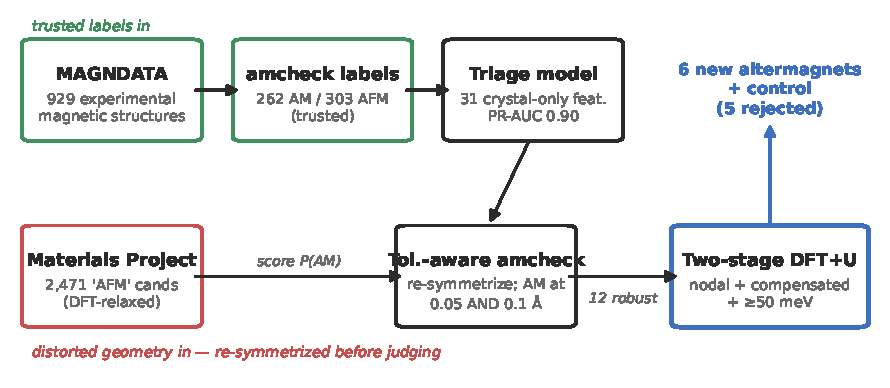
\includegraphics[width=\textwidth]{figures/fig1_pipeline.pdf}
\caption{\label{fig:pipeline}The discovery pipeline. Trusted experimental
labels (MAGNDATA, green) train the triage model; DFT-relaxed Materials Project
candidates (red) are scored, re-symmetrized, verified by tolerance-aware
\textit{amcheck}, and confirmed by two-stage DFT+$U$ (blue).}
\end{figure*}

\section{Methods}

\textit{Trusted training labels.} Materials are labeled altermagnet (AM) or
antiferromagnet (AFM) by applying \textit{amcheck}~\cite{Smolyanyuk2024} to
their magnetic structure. Training labels come only from
MAGNDATA~\cite{Gallego2016}, whose moments are experimentally determined: 929
commensurate entries yield 262~AM / 303~AFM after removing ferromagnetic and
symmetry-frustrated cases.

\textit{Leakage-free descriptors.} Each structure is described by 31
crystal-only features: composition-weighted element-property statistics plus
non-magnetic symmetry/geometry, computed with
pymatgen/spglib~\cite{Ong2013}. No feature derives from magnetic moments.
Symmetry features are computed at symprec $=0.1$~\AA{} to place DFT-relaxed
(Materials Project~\cite{Jain2013}) and experimental (MAGNDATA) structures on a
comparable footing (Sec.~\ref{sec:blindspot}).

\textit{Classifier.} A histogram gradient-boosted tree
(scikit-learn~\cite{Pedregosa2011}) with balanced class weights, evaluated by
stratified 5-fold cross-validation.

\textit{Candidate scoring and verification.} The trained model scores Materials
Project AFM structures. High-probability candidates are verified by re-running
\textit{amcheck} across symmetry tolerances ($10^{-3}$--$10^{-1}$~\AA); a
candidate is \textit{robust} when classified AM at both 0.05 and 0.1~\AA{}
(guarding against over-symmetrization).

\textit{First-principles confirmation.} Spin-polarized DFT+$U$
(\textsc{Quantum ESPRESSO} 7.3.1~\cite{Giannozzi2009}; PBE; Hubbard $U$ on
open-shell $d$ states: 4.5~eV Fe-3$d$, 3.5 Cr-3$d$, 4.0 Mn/Co-3$d$, 3.0 V-3$d$,
6.0 Cu-3$d$, 2.5 Mo-4$d$, 2.0 W-5$d$/Zr-4$d$; PAW pseudopotentials) with the
compensated collinear AFM configuration encoded by splitting each magnetic
element into two species of opposite starting magnetization. Correlated double
perovskites exhibit bistable SCF (competition with ferrimagnetic states);
convergence required pinning the compensated configuration via a
constrained-magnetization penalty (\texttt{constrained\_magnetization='atomic'},
$\lambda=0.5$) with Marzari--Vanderbilt smearing (0.03~Ry) and plain Broyden
mixing ($\beta=0.1$, history 20).

Confirmation criteria: (i)~momentum-dependent up/down splitting $\geq 50$~meV
within $\pm 3$~eV of $E_F$; (ii)~net moment $\leq 0.5\,\mu_B$/cell
(compensation); and (iii)~a \textit{nodal criterion}---the per-$k$ splitting
must fall below half its maximum somewhere on the path, since altermagnetic
symmetry requires nodal directions; large but $k$-uniform splitting at zero net
moment instead signals a compensated ferrimagnet. Calculations were run in two
stages: first-pass (ecut 45~Ry, $2{\times}2{\times}2$ charge $k$-mesh, conv
$5{\times}10^{-4}$~Ry) on all candidates, then refinement (ecut 60~Ry, ecutrho
480~Ry; $4{\times}4{\times}4$ $k$ for cells $\leq 18$ atoms,
$3{\times}3{\times}3$ for larger; conv $10^{-4}$--$10^{-5}$~Ry) on all
first-pass positives; only refinement-surviving materials are claimed. All
calculations ran on a single Apple M1~Max workstation using a natively compiled
\textsc{Quantum ESPRESSO}.

\section{Results}

\subsection{Label provenance dominates}

A model trained on Materials Project (DFT-derived, noisy) AM/AFM labels attains
reasonable cross-validation yet scores at chance (ROC-AUC 0.54) on the trusted
MAGNDATA set---a textbook distribution-shift failure
(Fig.~\ref{fig:provenance}). The identical features trained on trusted MAGNDATA
labels reach ROC-AUC 0.91 / PR-AUC 0.90. Trusted labels, not model capacity,
are decisive.

\begin{figure}
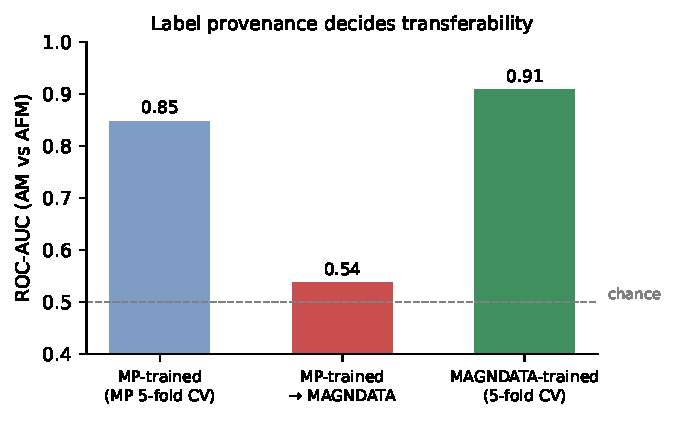
\includegraphics[width=\columnwidth]{figures/fig2_provenance.pdf}
\caption{\label{fig:provenance}Label provenance decides transferability.
MP-trained models collapse to chance on experimental structures; the same
features with trusted labels perform well.}
\end{figure}

\subsection{The tolerance blind spot, quantified}\label{sec:blindspot}

At the conventional $10^{-3}$~\AA{} tolerance, 63\% of Materials Project
candidates read as triclinic versus 0.2\% of experimental MAGNDATA
structures---a gross feature-distribution mismatch driven entirely by
relaxation distortions (Fig.~\ref{fig:blindspot}). Loosening to 0.1~\AA{}
reduces the MP triclinic fraction to 26\% and aligns the distributions. Case
studies confirm the mechanism: Sr$_2$FeWO$_6$ reads as triclinic/monoclinic at
$10^{-3}$~\AA{} but recovers its ideal double-perovskite symmetry---and an
altermagnetic classification---at 0.05--0.1~\AA.

\begin{figure*}
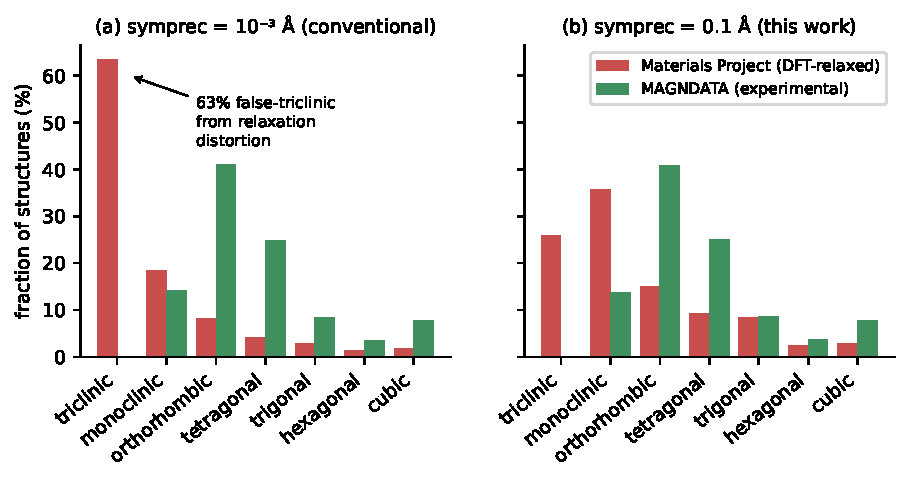
\includegraphics[width=\textwidth]{figures/fig3_blindspot.pdf}
\caption{\label{fig:blindspot}The tolerance blind spot. (a)~At symprec
$=10^{-3}$~\AA, DFT-relaxed structures read overwhelmingly as false-triclinic;
(b)~at 0.1~\AA{} the distributions align with experiment.}
\end{figure*}

\subsection{Validation against independent studies}

The pipeline's confirmed set overlaps prior DFT-confirmed altermagnets
(Fig.~\ref{fig:novelty}), including an exact-structure match with Gao
\textit{et al.}~\cite{Gao2025}: Ba$_2$CoSi$_2$O$_7$ (mp-510015), plus
compound-level matches LiFeF$_4$ and CaLaCrMoO$_6$. As a positive control, our
DFT setup reproduces CaLaCrMoO$_6$'s altermagnetism (210~meV splitting,
formally converged), independently validating the recipe applied to the novel
candidates.

\begin{figure}
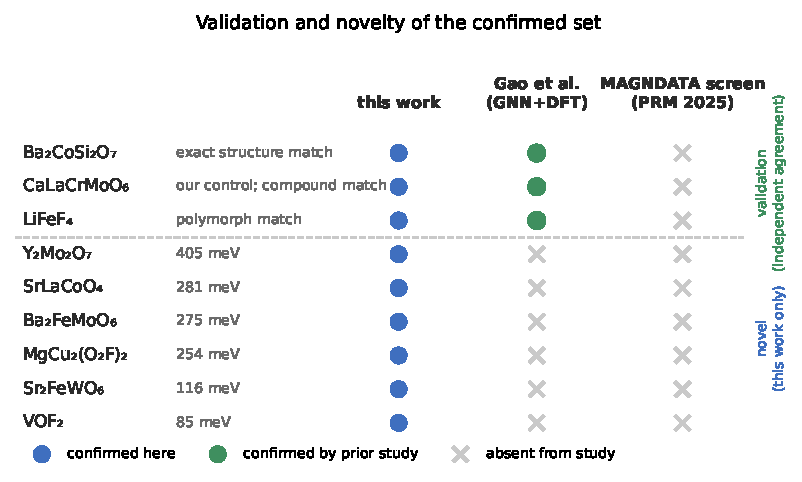
\includegraphics[width=\columnwidth]{figures/fig4_novelty.pdf}
\caption{\label{fig:novelty}Validation and novelty. Three overlaps with prior
studies validate the pipeline; six confirmed compounds are reported here for
the first time.}
\end{figure}

\subsection{Two-stage confirmation: six new altermagnets}

Table~\ref{tab:results} gives refined DFT+$U$ verdicts for all twelve
tolerance-robust candidates. Every confirmed material satisfies all three
criteria: splitting $\geq 50$~meV, net moment ${\approx}0$, and nodal
momentum-dependence (min per-$k$ splitting $\leq 10\%$ of max in all six;
Fig.~\ref{fig:dft}). Confirmed magnitudes shift by $\leq 25\%$ between
first-pass and refined settings, while verdicts for the six are unchanged. The
electronic classification splits the set into two metallic altermagnets---
SrLaCoO$_4$ and Ba$_2$FeMoO$_6$, natural candidates for
altermagnet/superconductor heterostructures and spin-transport experiments---
and four insulating ones suited to low-dissipation magnonic and tunnel-barrier
applications. (Gap values are indicative only: PBE+$U$ systematically
misestimates gap magnitudes, so the metal/insulator distinction is claimed, the
values are not.)

\begin{table*}
\caption{\label{tab:results}Refined DFT+$U$ verdicts for the twelve
tolerance-robust candidates (first-pass values in parentheses where
different).}
\begin{ruledtabular}
\begin{tabular}{llccccl}
Material & MP id & max split (meV) & per-$k$ range & net mom ($\mu_B$) & electronic & verdict\\
\hline
Y$_2$Mo$_2$O$_7$    & mp-2674749 & 405 (360) & 4--405    & $+0.01$ & ins.\ (${\sim}0.9$ eV) & \textbf{AM, new} (nodal)\\
SrLaCoO$_4$         & mp-1274449 & 281       & 11--281   & $-0.01$ & metal                  & \textbf{AM, new}\\
Ba$_2$FeMoO$_6$     & mp-1277787 & 275 (366) & 3--275    & $-0.00$ & metal                  & \textbf{AM, new} (nodal)\\
MgCu$_2$(O$_2$F)$_2$& mp-2240166 & 254 (269) & 5--254    & $-0.00$ & ins.\ (${\sim}0.4$ eV) & \textbf{AM, new}\\
CaLaCrMoO$_6$       & mp-1048863 & 210 (205) & 12--210   & $+0.01$ & ins.\ (${\sim}0.6$ eV) & AM (control \checkmark)\\
Sr$_2$FeWO$_6$      & mp-19266   & 116 (125) & 11--116   & $+0.00$ & ins.\ (${\sim}2.1$ eV) & \textbf{AM, new}\\
VOF$_2$             & mp-759163  & 85 (93)   & 1--85     & $+0.00$ & ins.\ (${\sim}1.7$ eV) & \textbf{AM, new} (nodal)\\
ZrCoO$_3$           & mp-756665  & 19 (115)  & 6--19     & $-0.00$ & ---                    & rejected at refinement\\
Ca$_3$Co$_2$O$_7$   & mp-1580697 & 758       & 390--758  & $-0.83$ & ---                    & rejected (magnetized)\\
Ba$_2$FeWO$_6$      & mp-1272506 & 1888 (232)& 1656--1888& $-0.00$ & ---                    & rejected (node-less; comp.\ FiM)\\
MnOF                & mp-1277241 & 30        & 24--30    & $+0.00$ & ---                    & rejected (sub-threshold)\\
CsTaCo(OF$_2$)$_2$  & mp-684727  & ---       & ---       & $+1.70$ & ---                    & rejected (ferrimagnetic)\\
\end{tabular}
\end{ruledtabular}
\end{table*}

\begin{figure*}
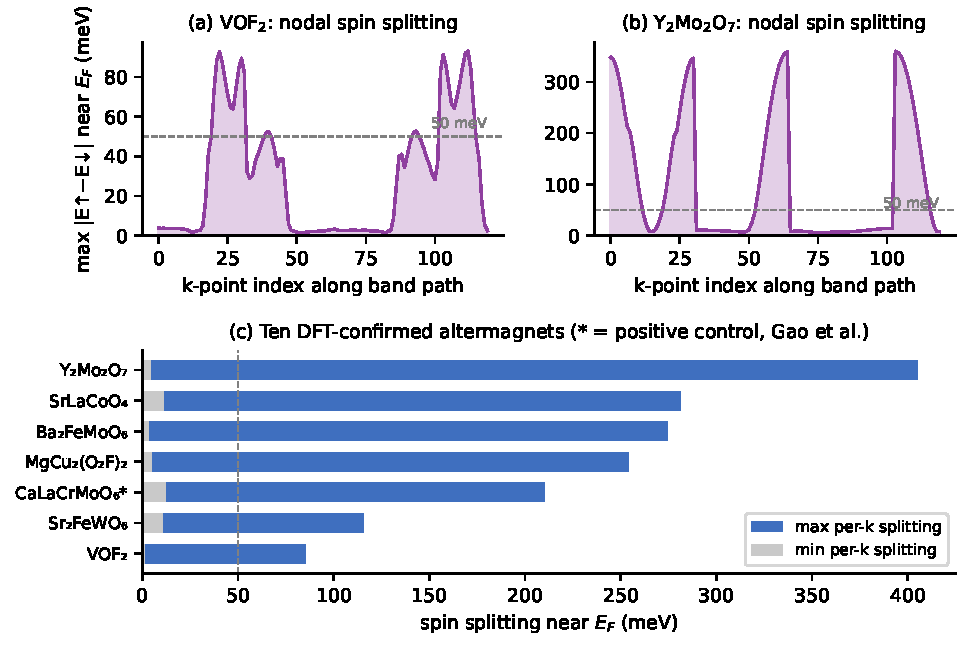
\includegraphics[width=\textwidth]{figures/fig5_dft.pdf}
\caption{\label{fig:dft}DFT confirmation. (a,b)~Per-$k$ spin splitting of
VOF$_2$ and Y$_2$Mo$_2$O$_7$ showing the nodal structure required by
altermagnetic symmetry; (c)~maximum and minimum per-$k$ splitting for the seven
confirmed materials.}
\end{figure*}

The five rejections trace a graded attrition that validates each filter stage.
MnOF is symmetry-permitted but electronically weak. CsTaCo(OF$_2$)$_2$ will not
hold a compensated state even under the magnetization constraint. ZrCoO$_3$'s
first-pass 115~meV collapses to 19~meV at refined numerics---a loose-settings
artifact caught by our own quality pass. Ca$_3$Co$_2$O$_7$ drifts to a
magnetized solution on the denser $k$-mesh. Most instructively,
Ba$_2$FeWO$_6$ develops a giant (1.9~eV) but nearly $k$-uniform splitting: the
absence of nodes identifies its refined ground state as a compensated
ferrimagnet, not an altermagnet. Symmetry analysis bounds what may occur;
two-stage DFT decides what does.

\subsection{Why prior screens missed these}

None of the six appears in Gao \textit{et al.}'s 50 confirmed
materials~\cite{Gao2025}, although both searches mine the same structural
families (their set contains the adjacent compositions Ca$_3$Cr$_2$O$_7$ and
ZrCrO$_3$, chromium analogues of two of our candidates). The most parsimonious
explanation is the distortion blind spot: methods that trust the as-relaxed
cell cannot see altermagnets whose defining rotation is broken only
numerically. An explicit re-symmetrization step---cheap and interpretable---
recovers them.

\section{Discussion}

The recurring lesson is that both failure modes we identified are
data-representation problems, not model-capacity problems: noisy DFT labels
destroy transferability, and numerically-distorted geometry hides the defining
symmetry. A simple classifier with trusted labels plus tolerance-aware
verification outperforms---in novel-material yield---a pre-trained GNN on the
same chemistry, because it corrects the representation rather than adding
capacity. We recommend that altermagnet screens evaluate symmetry across a
tolerance range, or symmetrize before classifying, rather than trusting a
single tight tolerance.

\textit{Configuration-specific claims.} Our calculations address the
compensated collinear AFM configuration catalogued by the Materials Project for
each compound. For Sr$_2$FeWO$_6$ this coincides with the experimentally
observed ground state (AFM insulator, $T_N \approx 37$~K). For
Ba$_2$FeMoO$_6$---whose family is known for half-metallic ferrimagnetism---and
Y$_2$Mo$_2$O$_7$---experimentally a frustrated pyrochlore spin glass---the
studied configuration is a competing order rather than the observed ground
state; realizing their altermagnetism would require stabilizing that
configuration (e.g.\ by strain, doping or field protocols). VOF$_2$ and
MgCu$_2$(O$_2$F)$_2$ are computationally predicted structures whose synthesis
remains to be established. All claims should be read as
configuration-specific.

\textit{Limitations.} Hubbard $U$ values are standard literature choices, not
material-specific fits, and the refined $k$-meshes remain modest by
converged-property standards; magnitudes may shift further at denser sampling,
though the $\leq 25\%$ first-pass$\to$refined drift for all six confirmed
materials suggests stability. N\'eel temperatures remain to be computed.
Wave-type classification ($d$/$g$/$i$) from the nodal patterns is left to
follow-up work.

\section{Conclusion}

An interpretable, trusted-data pipeline with tolerance-aware symmetry
verification and two-stage first-principles confirmation yields six new
DFT-confirmed altermagnets spanning four structural families, reproduces an
independently-confirmed control, and rejects five false candidates through
successively stricter physical criteria. The enabling insight---that
tight-tolerance symmetry screening systematically hides altermagnets in
slightly-distorted high-symmetry cells---is both a concrete list of new
materials and a methodological correction for the field.

\begin{acknowledgments}
Calculations were performed on a single Apple M1~Max workstation with a
natively compiled \textsc{Quantum ESPRESSO}. Pipeline code and data are
available at [Zenodo/GitHub DOI to be added].
\end{acknowledgments}

\begin{thebibliography}{12}

\bibitem{Smejkal2022beyond} L.~\v{S}mejkal, J.~Sinova, and T.~Jungwirth,
Beyond conventional ferromagnetism and antiferromagnetism: A phase with
nonrelativistic spin and crystal rotation symmetry,
Phys. Rev. X \textbf{12}, 031042 (2022).

\bibitem{Smejkal2022landscape} L.~\v{S}mejkal, J.~Sinova, and T.~Jungwirth,
Emerging research landscape of altermagnetism,
Phys. Rev. X \textbf{12}, 040501 (2022).

\bibitem{Krempasky2024} J.~Krempask\'y \textit{et al.},
Altermagnetic lifting of Kramers spin degeneracy,
Nature \textbf{626}, 517 (2024).

\bibitem{Smolyanyuk2024} A.~Smolyanyuk, L.~\v{S}mejkal, and I.~I. Mazin,
A tool to check whether a symmetry-compensated collinear magnetic material is
antiferro- or altermagnetic, SciPost Phys. Codebases \textbf{30} (2024),
doi:10.21468/SciPostPhysCodeb.30.

\bibitem{PRM2025screen} High-throughput screening of altermagnetic materials,
Phys. Rev. Materials \textbf{9}, 064403 (2025); High-throughput quantification
of altermagnetic band splitting, Phys. Rev. Materials (2025),
doi:10.1103/mmdm-hrj4.

\bibitem{Gao2025} Z.-F. Gao, S.~Qu, B.~Zeng, Y.~Liu, J.-R. Wen, H.~Sun,
P.-J. Guo, and Z.-Y. Lu, AI-accelerated discovery of altermagnetic materials,
Natl. Sci. Rev. \textbf{12}, nwaf066 (2025).

\bibitem{Naka2025} M.~Naka, Y.~Motome, and H.~Seo, Altermagnetic perovskites,
npj Spintronics \textbf{3}, 1 (2025).

\bibitem{Gallego2016} S.~V. Gallego \textit{et al.}, MAGNDATA: towards a
database of magnetic structures. I.~The commensurate case,
J. Appl. Cryst. \textbf{49}, 1750 (2016).

\bibitem{Jain2013} A.~Jain \textit{et al.}, The Materials Project: A materials
genome approach to accelerating materials innovation,
APL Mater. \textbf{1}, 011002 (2013).

\bibitem{Giannozzi2009} P.~Giannozzi \textit{et al.}, QUANTUM ESPRESSO: a
modular and open-source software project for quantum simulations of materials,
J. Phys.: Condens. Matter \textbf{21}, 395502 (2009); \textbf{29}, 465901
(2017).

\bibitem{Ong2013} S.~P. Ong \textit{et al.}, Python Materials Genomics
(pymatgen), Comput. Mater. Sci. \textbf{68}, 314 (2013); A.~Togo and
I.~Tanaka, spglib, arXiv:1808.01590.

\bibitem{Pedregosa2011} F.~Pedregosa \textit{et al.}, Scikit-learn: Machine
learning in Python, J. Mach. Learn. Res. \textbf{12}, 2825 (2011).

\end{thebibliography}

\end{document}
